\documentclass[12pt, a4paper]{ctexart}

% 页面边距设置
\usepackage[left=2.5cm, right=2.5cm, top=2.5cm, bottom=2.5cm]{geometry}

% 常用宏包
\usepackage{graphicx}      % 图片支持
\usepackage{hyperref}      % 超链接
\usepackage{booktabs}      % 三线表
\usepackage{longtable}     % 长表格
\usepackage{array}         % 数组表格增强
\usepackage{xcolor}        % 颜色支持
\usepackage{listings}      % 代码块支持
\usepackage{amsmath}       % 数学公式
\usepackage{amssymb}       % 数学符号（\checkmark, \square 等）
\usepackage{tcolorbox}     % 文本框/高亮块

% 超链接设置
\hypersetup{
    colorlinks=true,
    linkcolor=blue,
    filecolor=magenta,      
    urlcolor=cyan,
}

% 代码块样式设置
\lstset{
    basicstyle=\ttfamily\small,
    breaklines=true,
    frame=single,
    backgroundcolor=\color{gray!10},
    language=Python, % 默认语言，可根据需要调整
}

% 标题信息
\title{\textbf{MathMate 说明文档}}
\author{项目报告}
\date{\today}

\begin{document}

\maketitle
\thispagestyle{empty} % 封面页不显示页码
\setcounter{page}{1} % 从正文开始计数

% 封面页表格
\begin{center}
\renewcommand{\arraystretch}{1.5}
\begin{tabular}{ll}
\textbf{项目} & \textbf{内容} \\
\textbf{作品名称} & MathMate - 智能数学学习助手 \\
\textbf{参赛赛道} & 开放赛道 \\
\textbf{选手姓名} & 马兆坤\qquad 章开元\qquad 丁宇鑫\qquad 周星橙\qquad 应沛成 \\
\textbf{Demo 链接} & （待填写） \\
\end{tabular}
\end{center}

\newpage
\tableofcontents % 目录
\newpage

% 模块一
\section{模块一：用户洞察与问题定义}

\subsection{目标用户}
MathMate 面向 \textbf{初中至高中阶段的学生}（12-18 岁），兼顾大学生及数学自学者。用户画像特征：
\begin{itemize}
    \item 日常有数学刷题需求，遇到难题缺乏即时解答渠道
    \item 传统搜题 App 仅提供答案，缺乏解题思路讲解和图形化理解
    \item 对几何、函数等抽象概念需要可视化辅助理解
    \item 偏好移动端学习，习惯碎片化时间刷题
\end{itemize}

\subsection{用户痛点}
\begin{enumerate}
    \item \textbf{拍题只给答案，不讲思路}：市面拍照搜题产品多为题库匹配，只输出最终答案和固定解析，无法针对性地解释学生困惑的点；遇到题库未收录的题目则完全无能为力。
    \item \textbf{几何题目难以可视化理解}：静态的题目图片无法展示几何图形的动态关系（如动点轨迹、切线变化），学生难以建立空间直觉。传统搜题产品不提供交互式几何图形。
    \item \textbf{学习工具分散}：学生需要在多个 App 之间切换——计算器、画图工具、搜题工具、笔记工具，学习流程被打断，效率低下。
    \item \textbf{缺乏个性化辅导}：不同年级、不同水平的学生需要不同深度和风格的讲解，但传统搜题产品千人一面。
\end{enumerate}

\subsection{使用场景}
\subsubsection{场景一：晚自习遇到难题}
高三学生小张在晚自习刷数学卷子，遇到一道解析几何大题不会做。他打开 MathMate，拍照上传题目。10 秒内，App 完成了题目识别、AI 求解，并自动生成了一道交互式几何图形——他可以拖动图上的动点，直观看到轨迹变化和临界条件。同时 AI 给出了分步骤的解题思路，从审题、建模到计算、验证全程展示。小张看完后理解了这类题的通用解法，将解题过程收藏到历史记录。

\subsubsection{场景二：考前专题复习}
初三学生小李在备考二次函数专题，对函数图像平移、开口方向、与 x 轴交点等概念感到困惑。她打开 MathMate 的 AI 聊天助手，用自然语言提问：“二次函数 $y=ax^2+bx+c$ 中 $a$ 的正负和大小到底怎么影响图像？”AI 助手即时回复了解释，并调用了函数绘图工具实时展示不同参数下的图像变化。小李还浏览了 App 推荐的 B 站数学视频，找到了 3Blue1Brown 风格的可视化解说，彻底理解了函数变换。

% 模块二
\section{模块二：产品方案设计}

\subsection{产品概述}
MathMate 是一款 \textbf{以 AI 大模型为核心驱动} 的智能数学学习移动应用。它深度融合了多模态 AI（图片识别、自然语言理解、数学推理）与交互式数学可视化（GeoGebra、自研几何渲染引擎），为学生提供「拍照搜题 $\rightarrow$ AI 分步讲解 $\rightarrow$ 交互式几何可视化 $\rightarrow$ 个性化对话辅导」的一站式数学学习体验。

\subsection{核心功能}
\begin{center}
\begin{tabular}{|p{3cm}|p{3.5cm}|p{5cm}|}
\hline
\textbf{功能模块} & \textbf{解决的问题} & \textbf{核心实现} \\ \hline
拍照搜题 + AI 求解 & 遇到难题没有即时解答 & 多模态 AI 识别题目 $\rightarrow$ DeepSeek 大模型分步求解 \\ \hline
交互式几何可视化 & 几何题目抽象难懂 & AI 生成几何 JSON $\rightarrow$ Canvas 自研引擎渲染可交互图形 \\ \hline
AI 对话助手 & 学习中的个性化疑问 & 流式聊天 LLM，支持上下文多轮对话、公式实时渲染 \\ \hline
数学工具箱 & 画图、计算需切换多个 App & 集成 GeoGebra（6 种工具：科学计算器、几何画板、函数绘图、3D 视图、尺规作图、概率模型） \\ \hline
智能视频推荐 & 不知道该看什么学习资源 & AI 推荐 + 历史记录分析 $\rightarrow$ B 站数学视频精准推荐 \\ \hline
手写笔记 & 需要手写推导过程 & 支持多种纸张背景的手写笔记与富文本编辑器 \\ \hline
\end{tabular}
\end{center}

\newpage
\subsection{产品架构图}
\begin{figure}[htbp]
    \centering
    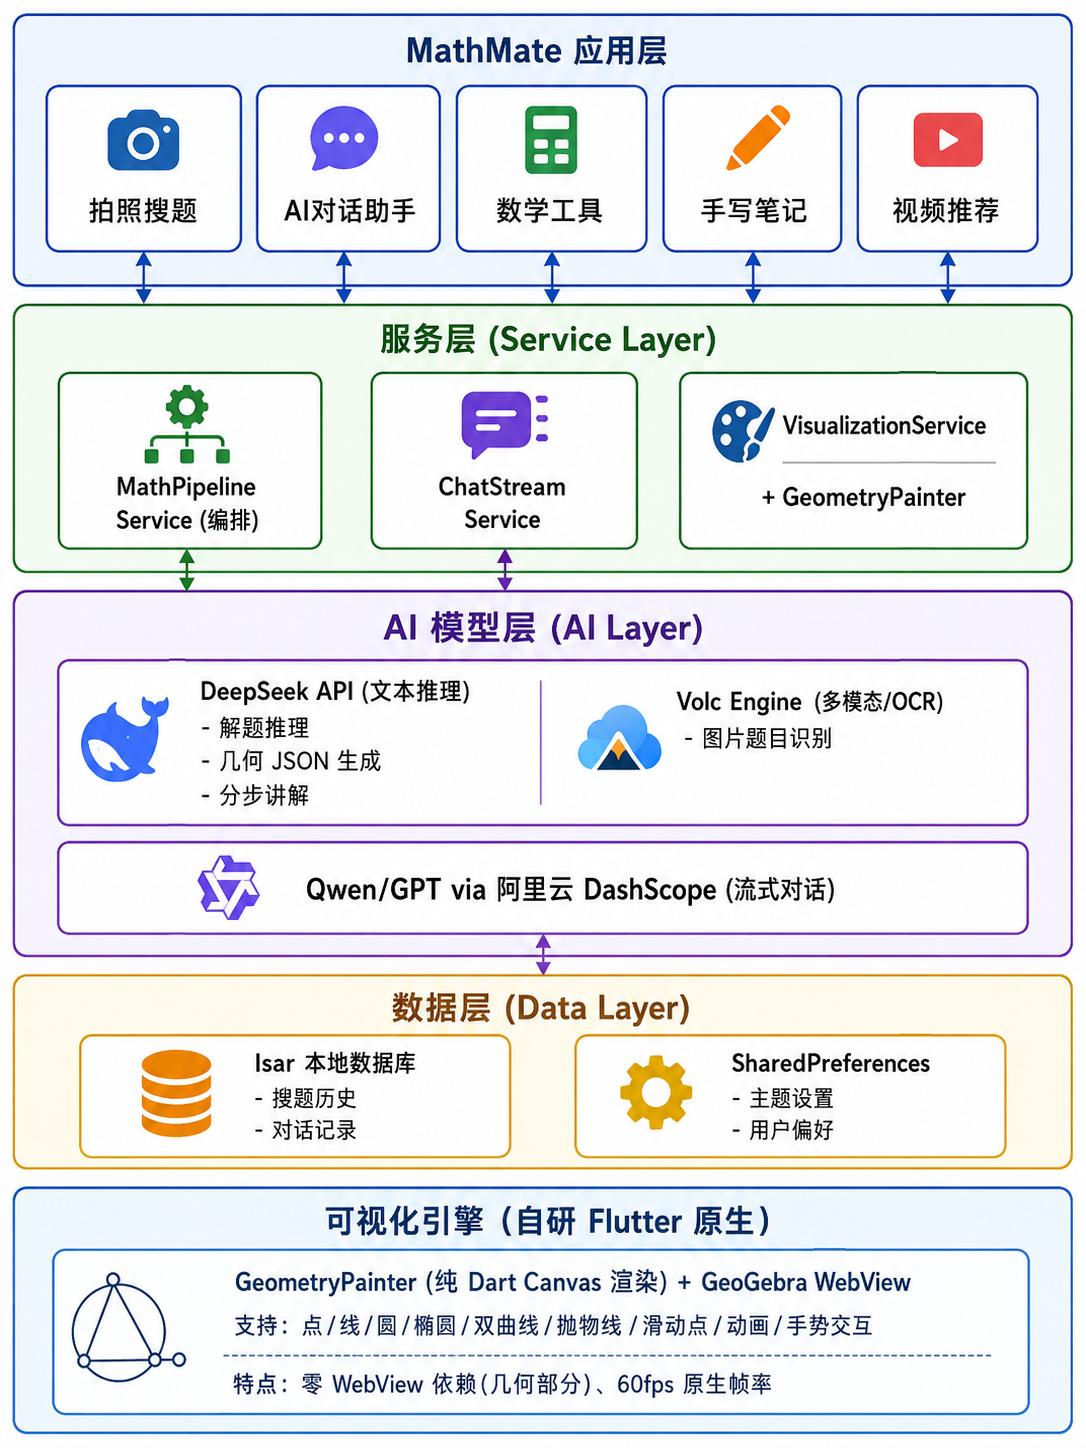
\includegraphics[width=\textwidth]{image1.png}
    \caption{产品架构图}
    \label{fig:image1}
\end{figure}


\subsection{交互流程}
\textbf{核心流程：拍照搜题 $\rightarrow$ 结果展示}
\begin{figure}[htbp]
    \centering
    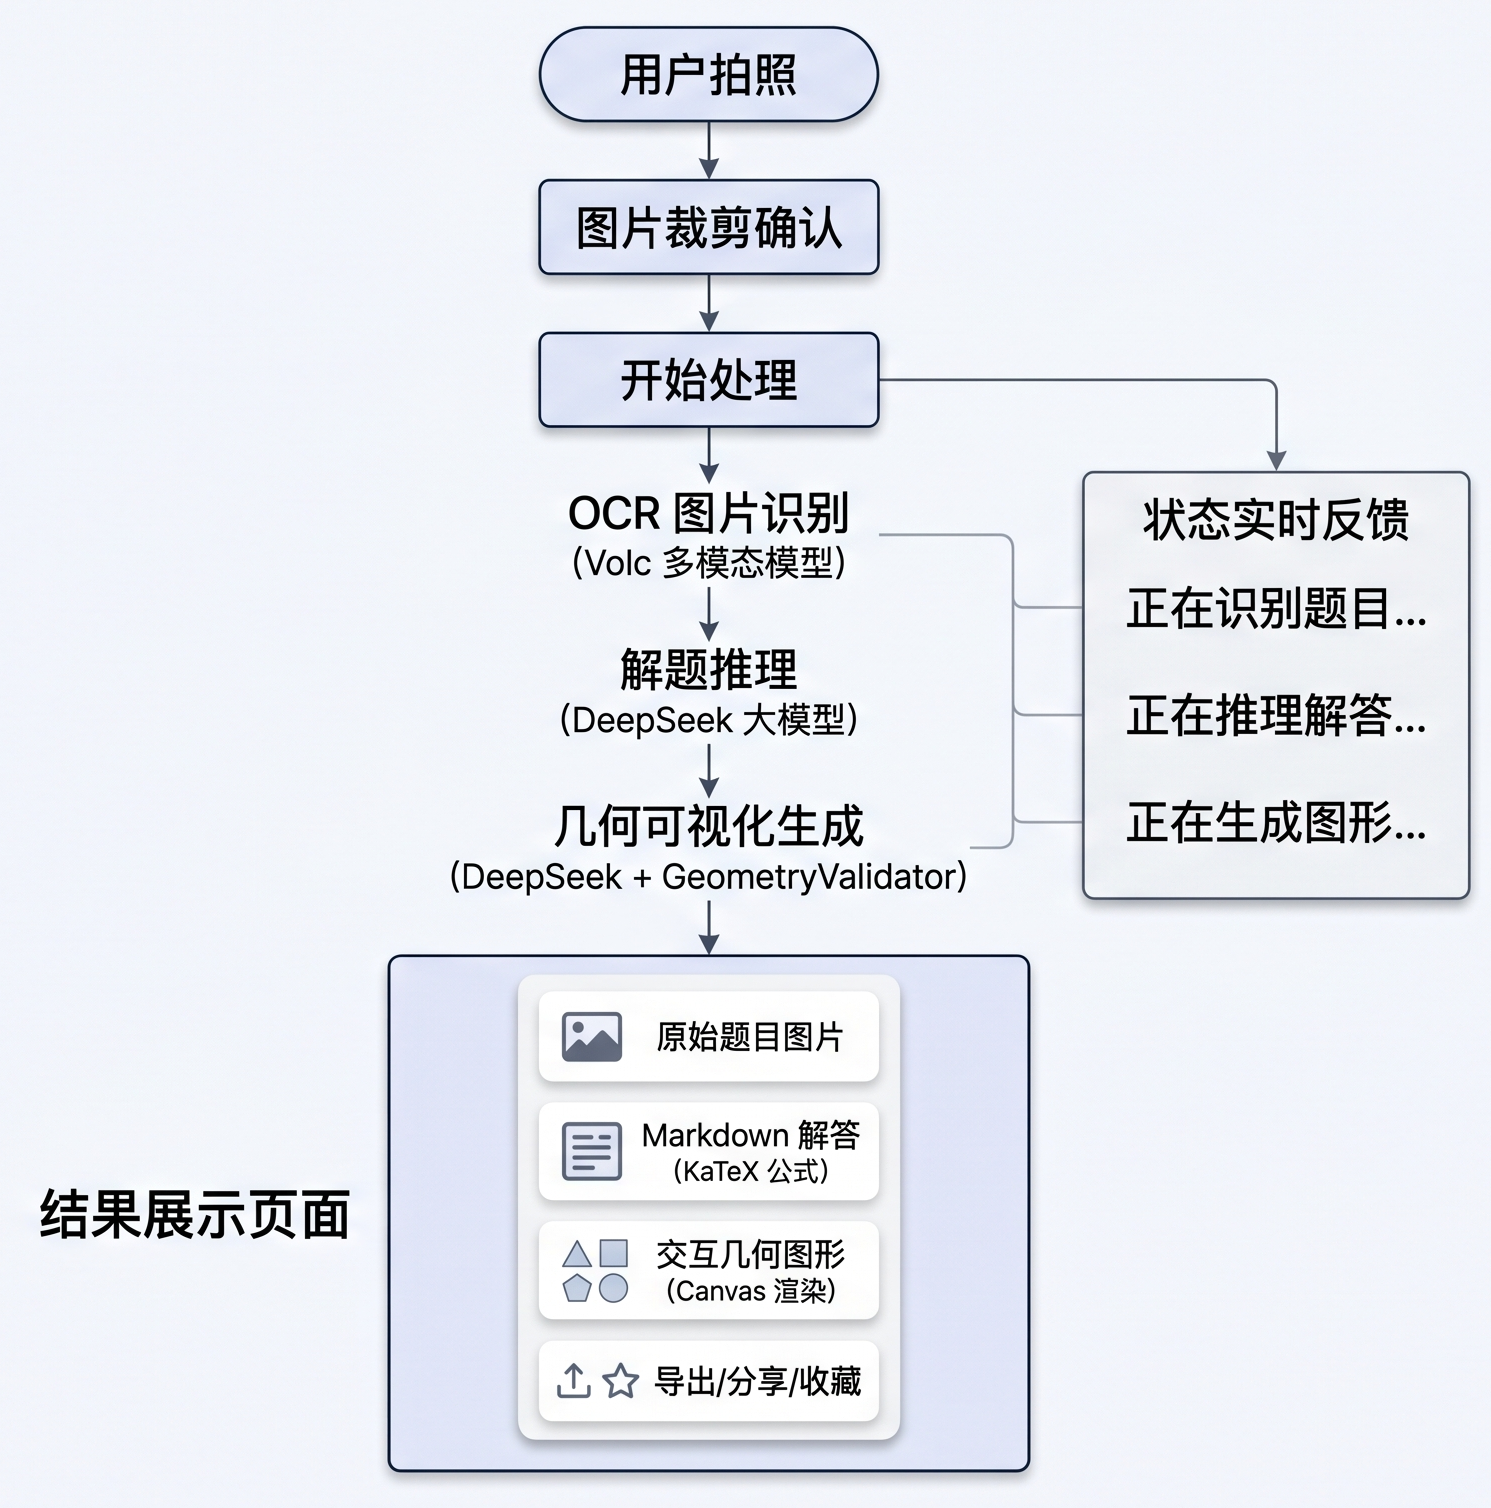
\includegraphics[width=\textwidth]{image2.png}
    \caption{交互流程}
    \label{fig:image2}
\end{figure}

\subsection{创新与差异化}
\begin{center}
\begin{tabular}{|p{2cm}|p{5cm}|p{5cm}|}
\hline
\textbf{对比维度} & \textbf{传统搜题 App（作业帮等）} & \textbf{MathMate} \\ \hline
\textbf{解题方式} & 题库匹配 $\rightarrow$ 返回固定解析 & AI 实时推理 $\rightarrow$ 动态生成分步讲解 \\ \hline
\textbf{几何可视化} & 静态图片或无图形 & AI 自动生成交互式几何图形，可拖拽探索 \\ \hline
\textbf{题目覆盖} & 仅限题库收录的题目 & 无题库限制，任意题目均可识别并求解 \\ \hline
\textbf{学习工具} & 单一搜题功能 & 一站式：搜题 + 对话辅导 + 工具箱 + 视频推荐 \\ \hline
\textbf{个性化} & 无差异化 & 按年级分层，AI 对话支持多轮追问 \\ \hline
\textbf{图形技术} & 无或简单图片 & \textbf{自研 Flutter 原生可视化引擎}，纯 Dart + Canvas 实现，零 WebView 依赖，支持点/线/圆/椭圆/双曲线/抛物线/动点动画/拖拽交互 \\ \hline
\end{tabular}
\end{center}

% 模块三
\section{模块三：AI 原生能力说明}

\subsection{AI 核心能力}
MathMate 的核心是一个 \textbf{多模型协作的 AI 流水线}，使用了以下 AI 能力：
\begin{center}
\begin{tabular}{|p{4cm}|p{4cm}|p{4cm}|}
\hline
\textbf{AI 能力} & \textbf{应用场景} & \textbf{所用模型/API} \\ \hline
多模态理解（视觉识别） & 拍照后将手写/印刷数学题转为 Markdown & Volc Engine 多模态模型 \\ \hline
大模型数学推理 & 对识别出的数学题进行分步推理解答 & DeepSeek API \\ \hline
大模型结构化输出 & 根据题目和解答生成几何图形 JSON & DeepSeek API \\ \hline
大模型流式对话 & AI 问答助手的多轮自然语言交互 & 阿里云 DashScope (Qwen-PLUS) \\ \hline
AI 视频推荐 & 根据用户搜索历史推荐学习视频 & DeepSeek API \\ \hline
\end{tabular}
\end{center}

\subsection{AI 如何解决痛点}
\textbf{问：去掉 AI，这个产品还能成立吗？}

\textbf{不能。} MathMate 的每一项核心功能都深度依赖 AI：
\begin{itemize}
    \item \textbf{拍照搜题}：没有 AI 多模态识别 $\rightarrow$ 手写题目无法数字化；没有 AI 推理 $\rightarrow$ 题库外题目无法求解。传统题库方案覆盖率和灵活性远不及大模型。
    \item \textbf{几何可视化}：几何图形的参数（位置、形状、动画）由 AI 从题目文本中自动抽取并结构化输出。去掉 AI，几何图形需要人工逐题编写，不具备可扩展性。
    \item \textbf{AI 对话助手}：自然语言理解 + 多轮数学推理是 LLM 的核心能力，没有任何传统方法可以替代。
    \item \textbf{视频推荐}：基于 DeepSeek 对用户学习和历史行为的语义理解进行推荐，而非简单的关键词匹配。
\end{itemize}

\textbf{AI 与痛点的绑定关系：}
\begin{itemize}
    \item 搜题不够灵活 $\rightarrow$ 大模型推理 $\rightarrow$ 任意题目均可实时求解
    \item 几何图形无法交互 $\rightarrow$ 大模型结构化输出 $\rightarrow$ AI 自动生成图形参数 JSON
    \item 缺乏个性化讲解 $\rightarrow$ LLM 多轮对话 $\rightarrow$ 针对性追问，适配不同水平
    \item 学习工具分散 $\rightarrow$ 多模型协作流水线 $\rightarrow$ 统一集成在一个 App 中
\end{itemize}

\newpage
\subsection{AI 技术方案}
\textbf{模型架构：多模型分层协作}
\begin{figure}[htbp]
    \centering
    \includegraphics[width=0.8\textwidth]{image3.png}
    \caption{模型架构图}
    \label{fig:image3}
\end{figure}



\textbf{AI 工作流详解（拍照搜题流水线）：}
\begin{enumerate}
    \item \textbf{OCR 识别阶段}（\texttt{OcrService}）
    \begin{itemize}
        \item 输入：用户拍摄/裁剪的题目图片
        \item 调用 Volc Engine 多模态 API，Prompt 指示模型将图片中的数学题转为 Markdown + LaTeX 格式
        \item 输出：结构化题目文本（含 LaTeX 公式）
    \end{itemize}
    \item \textbf{解题推理阶段}（\texttt{SolverService}）
    \begin{itemize}
        \item 输入：上一步的 Markdown 题目文本
        \item 调用 DeepSeek API，使用专用解题 Prompt（引导模型分步骤、详细讲解）
        \item 输出：Markdown 格式的分步解答（含 LaTeX 公式）
    \end{itemize}
    \item \textbf{几何可视化阶段}（\texttt{VisualizationService} + 自研渲染引擎）
    \begin{itemize}
        \item 输入：题目 + 解答的完整文本
        \item 调用 DeepSeek API，使用可视化专用 Prompt（指示模型输出 JSON 格式的几何场景描述，包含视口、点、线、圆、椭圆、双曲线、抛物线、动点等图元）
        \item 输出：经过 \texttt{GeometryValidator} 校验的结构化 JSON
        \item 渲染：\textbf{自研 Flutter 原生可视化引擎} \texttt{GeometryPainter} —— 纯 Dart 语言 + Flutter Canvas 实现，完全不依赖 WebView 或第三方图表库。直接从 JSON 解析为原生 Widget，在 Canvas 上绘制几何图形，支持动点轨迹动画（\texttt{AnimationController} 驱动）、滑块拖拽交互、无限直线视口裁剪、多图元混合渲染。相比 WebView 方案（如 GeoGebra/ECharts 嵌入），帧率更高、内存更低、交互零延迟
    \end{itemize}
\end{enumerate}

\textbf{技术选型理由：}
\begin{itemize}
    \item \textbf{DeepSeek} 作为核心推理引擎：在数学推理任务上表现优异，API 成本低，支持中文
    \item \textbf{Volc Engine} 处理视觉识别：多模态 OCR 精度高，对中文数学公式识别效果好
    \item \textbf{Qwen-PLUS} 处理流式对话：通过兼容 OpenAI 格式的 API 接入，延迟低，适合实时聊天
    \item \textbf{自研 Flutter 原生几何渲染引擎}：完全基于 Flutter Canvas + CustomPainter 实现，无需嵌入 WebView 即可渲染复杂数学几何图形。核心优势：(1) 原生级帧率（60fps），动画流畅无卡顿；(2) 零额外依赖，包体积远小于 WebView 方案；(3) 与 Flutter Widget 树无缝集成，支持手势拖拽、缩放等原生交互；(4) 纯 Dart 实现便于跨平台一致体验
\end{itemize}

% 模块四
\section{模块四：可行性分析}

\subsection{落地可行性}
\textbf{技术实现路径：}
\begin{center}
\begin{tabular}{|p{2cm}|p{6cm}|p{3cm}|}
\hline
\textbf{阶段} & \textbf{内容} & \textbf{状态} \\ \hline
Phase 1 & 核心流水线（OCR + 解题 + 可视化）、基础 UI 框架 & $\checkmark$ 已完成 (v1.2.0) \\ \hline
Phase 2 & AI 对话助手、流式响应、历史记录 & $\checkmark$ 已完成 \\ \hline
Phase 3 & GeoGebra 工具箱集成、手写笔记 & $\checkmark$ 已完成 \\ \hline
Phase 4 & 视频推荐系统、PDF 查看器 & $\checkmark$ 已完成 \\ \hline
Phase 5 & 跨平台完善（Windows/macOS/Linux）、性能优化 & $\circlearrowright$ 进行中 \\ \hline
Phase 6 & 个人知识图谱、错题本、智能复习规划 & $\square$ 规划中 \\ \hline
\end{tabular}
\end{center}

\textbf{技术栈成熟度：}
\begin{itemize}
    \item Flutter 跨平台框架：成熟稳定，一套代码覆盖 Android/iOS/Desktop
    \item DeepSeek / 阿里云 DashScope API：商用可用，有成熟的 SDK 和文档
    \item Isar 本地数据库：高性能、支持索引和查询，适合移动端
    \item GeoGebra WebView：世界领先的数学工具，提供完整 Web 组件
\end{itemize}

\textbf{所需资源评估：}
\begin{itemize}
    \item 开发：1-2 名 Flutter 开发者
    \item AI API 成本：每千次调用约 ¥20-50（取决于模型和 token 消耗），可规模化
    \item 无服务端成本：采用 Serverless 架构，AI 调用直接从客户端发起
\end{itemize}

\subsection{商业化思考}
\textbf{盈利模式：}
\begin{enumerate}
    \item \textbf{Freemium 模式（核心）}：
    \begin{itemize}
        \item 免费：每日限定次数的拍照搜题、基础 AI 对话
        \item 订阅会员：无限搜题、高级模型（更长推理链）、错题本、知识图谱、视频下载缓存
        \item 定价参考：¥19.9/月 或 ¥168/年
    \end{itemize}
    \item \textbf{B2B 合作}：
    \begin{itemize}
        \item 与教培机构合作，提供定制化的 AI 数学助教系统
        \item 为学校提供班级版产品，教师可查看班级学情数据
        \item API 授权：将核心 AI 求解能力封装为 API，供第三方教育产品调用
    \end{itemize}
\end{enumerate}

\end{document}